\documentclass[man, fleqn, noextraspace,floatsintext]{apa6}
\usepackage{lmodern}
\usepackage{amssymb,amsmath}
\usepackage{ifxetex,ifluatex}
\usepackage{fixltx2e} % provides \textsubscript
\ifnum 0\ifxetex 1\fi\ifluatex 1\fi=0 % if pdftex
  \usepackage[T1]{fontenc}
  \usepackage[utf8]{inputenc}
\else % if luatex or xelatex
  \ifxetex
    \usepackage{mathspec}
  \else
    \usepackage{fontspec}
  \fi
  \defaultfontfeatures{Ligatures=TeX,Scale=MatchLowercase}
\fi
% use upquote if available, for straight quotes in verbatim environments
\IfFileExists{upquote.sty}{\usepackage{upquote}}{}
% use microtype if available
\IfFileExists{microtype.sty}{%
\usepackage{microtype}
\UseMicrotypeSet[protrusion]{basicmath} % disable protrusion for tt fonts
}{}
\usepackage{hyperref}
\hypersetup{unicode=true,
            pdftitle={Effect of Gender and Socioeconomic Status on Math Score},
            pdfauthor={Jessica Canfield~\& Woocheol Kim},
            pdfkeywords={math scores, gender, socioeconomic status, teacher experience},
            pdfborder={0 0 0},
            breaklinks=true}
\urlstyle{same}  % don't use monospace font for urls
\usepackage{graphicx,grffile}
\makeatletter
\def\maxwidth{\ifdim\Gin@nat@width>\linewidth\linewidth\else\Gin@nat@width\fi}
\def\maxheight{\ifdim\Gin@nat@height>\textheight\textheight\else\Gin@nat@height\fi}
\makeatother
% Scale images if necessary, so that they will not overflow the page
% margins by default, and it is still possible to overwrite the defaults
% using explicit options in \includegraphics[width, height, ...]{}
\setkeys{Gin}{width=\maxwidth,height=\maxheight,keepaspectratio}
\IfFileExists{parskip.sty}{%
\usepackage{parskip}
}{% else
\setlength{\parindent}{0pt}
\setlength{\parskip}{6pt plus 2pt minus 1pt}
}
\setlength{\emergencystretch}{3em}  % prevent overfull lines
\providecommand{\tightlist}{%
  \setlength{\itemsep}{0pt}\setlength{\parskip}{0pt}}
\setcounter{secnumdepth}{0}
% Redefines (sub)paragraphs to behave more like sections
\ifx\paragraph\undefined\else
\let\oldparagraph\paragraph
\renewcommand{\paragraph}[1]{\oldparagraph{#1}\mbox{}}
\fi
\ifx\subparagraph\undefined\else
\let\oldsubparagraph\subparagraph
\renewcommand{\subparagraph}[1]{\oldsubparagraph{#1}\mbox{}}
\fi

%%% Use protect on footnotes to avoid problems with footnotes in titles
\let\rmarkdownfootnote\footnote%
\def\footnote{\protect\rmarkdownfootnote}


  \title{Effect of Gender and Socioeconomic Status on Math Score}
    \author{Jessica Canfield~\& Woocheol Kim\textsuperscript{1}}
    \date{}
  
\shorttitle{Research Article}
\affiliation{
\vspace{0.5cm}
\textsuperscript{1} University of Oregon}
\keywords{math scores, gender, socioeconomic status, teacher experience}
\usepackage{csquotes}
\usepackage{upgreek}
\captionsetup{font=singlespacing,justification=justified}

\usepackage{longtable}
\usepackage{lscape}
\usepackage{multirow}
\usepackage{tabularx}
\usepackage[flushleft]{threeparttable}
\usepackage{threeparttablex}

\newenvironment{lltable}{\begin{landscape}\begin{center}\begin{ThreePartTable}}{\end{ThreePartTable}\end{center}\end{landscape}}

\makeatletter
\newcommand\LastLTentrywidth{1em}
\newlength\longtablewidth
\setlength{\longtablewidth}{1in}
\newcommand{\getlongtablewidth}{\begingroup \ifcsname LT@\roman{LT@tables}\endcsname \global\longtablewidth=0pt \renewcommand{\LT@entry}[2]{\global\advance\longtablewidth by ##2\relax\gdef\LastLTentrywidth{##2}}\@nameuse{LT@\roman{LT@tables}} \fi \endgroup}

\authornote{\href{mailto:jcanfiel@uoregon.edu}{\nolinkurl{jcanfiel@uoregon.edu}}, Lundquist College of Business.

\href{mailto:wkim4@uoregon.edu}{\nolinkurl{wkim4@uoregon.edu}}, Lundquist College of Business.

We would like to thank Professor Joseph Nese and participants at 2019 International Educational Associations Conference for helpful comments.

Correspondence concerning this article should be addressed to Jessica Canfield, 1208 University of Oregon, Eugene, OR 97403. E-mail: \href{mailto:jcanfiel@uoregon.edu}{\nolinkurl{jcanfiel@uoregon.edu}}}

\abstract{
This paper reveals \textbf{gender} and \textbf{socioeconomic status} influence academic achievement, especially \textbf{math scores}. Along the way, it turns out that \textbf{teacher experience} is positively related to math scores such that the more teaching experience teachers have, the higher math scores students get.


}

\begin{document}
\maketitle

\hypertarget{introduction-and-overview}{%
\section{Introduction and Overview}\label{introduction-and-overview}}

Guo et al. (2015) explore expectancy value in mathematics, gender and socioeconomic background as predictors of achievement. A multi-cohort study is used in the research (see Guo et al., 2015). Stoet and Geary (2018) connects math with gender equality. Some other researchers study a similar topic. (see Stoet \& Geary, 2018). Quinn and Cooc (2015) take these topics further by creating a model that predicts science achievement gaps by gender and race.

\hypertarget{methods}{%
\section{Methods}\label{methods}}

We report how we determined our sample size, all data exclusions (if any), all manipulations, and all measures in the study.

\hypertarget{data-analysis}{%
\subsection{Data analysis}\label{data-analysis}}

\begin{table}[H]
\centering\begingroup\fontsize{15}{17}\selectfont

\begin{tabular}{l|l|r|r|r|r}
\hline
sex & frl & math\_mean & math\_sd & rdg\_mean & rdg\_sd\\
\hline
boy & no & 492.85 & 46.34 & 441.46 & 32.32\\
\hline
boy & yes & 469.87 & 46.09 & 425.38 & 26.63\\
\hline
girl & no & 501.21 & 45.96 & 448.54 & 34.52\\
\hline
girl & yes & 477.51 & 46.30 & 430.80 & 27.42\\
\hline
\end{tabular}
\endgroup{}
\end{table}

As we can see above, girls perform better than boys in both math and reading. Regardless of gender, students who do not receive free lunch get higher average scores in both math and reading than students who receive free lunch.

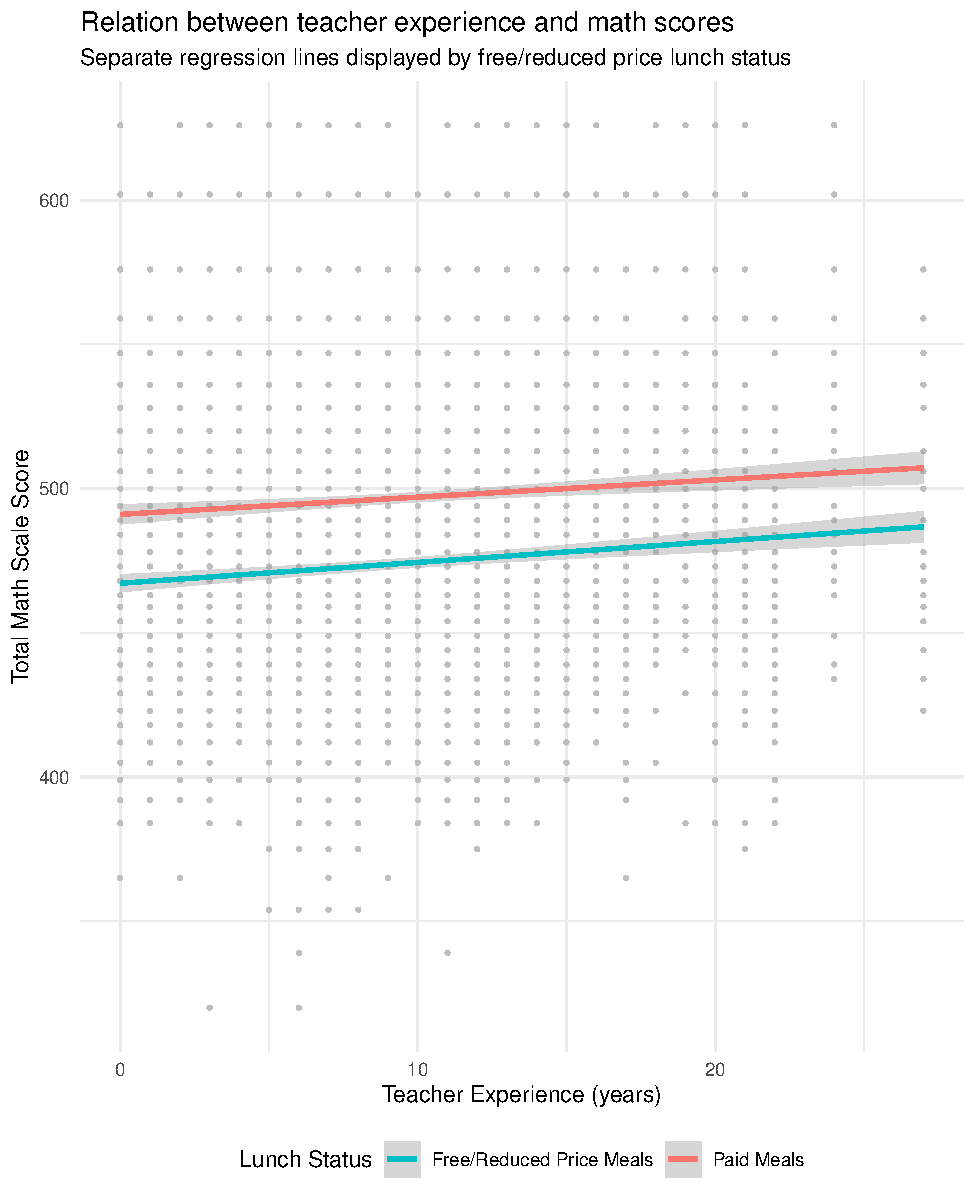
\includegraphics{lab_8_edld610_files/figure-latex/summary graph-1.pdf}

Teacher experience has a weak positive relationship with math scores and it is true for both free/reduced meal students and paid meal students.

\newpage

\hypertarget{references}{%
\section{References}\label{references}}

\begingroup
\setlength{\parindent}{-0.5in}
\setlength{\leftskip}{0.5in}

\hypertarget{refs}{}
\leavevmode\hypertarget{ref-guo_et_al_2015}{}%
Guo, J., Marsh, H. W., Parker, P. D., Morin, A. J., \& Yeung, A. S. (2015). Expectancy-value in mathematics, gender and socioeconomic background as predictors of achievement and aspirations: A multi-cohort study. \emph{Learning and Individual Differences}, \emph{37}, 161--168.

\leavevmode\hypertarget{ref-quinn_cooc_2015}{}%
Quinn, D. M., \& Cooc, N. (2015). Science achievement gaps by gender and race/ethnicity in elementary and middle school: Trends and predictors. \emph{Educational Researcher}, \emph{44}(6), 336--346.

\leavevmode\hypertarget{ref-stoet_geary_2018}{}%
Stoet, G., \& Geary, D. C. (2018). The gender-equality paradox in science, technology, engineering, and mathematics education. \emph{Psychological Science}, \emph{29}(4), 581--593.

\endgroup


\end{document}
